\section{Case study}
\label{sec:case}
In this section a real life application of OMERF method is analysed, comparing its performance with that of the models already presented in Section \ref{sec:sim}.
The data used concern 427 students of a prestigious high school in Milan, containing  all the personal information stored in the school's electronic register.
The objective of this section is to explore and analyse potential approaches used to predict students' academic achievements and search the factors influencing these outcomes.
The final aim is to identify students who may be at risk of failure and generally to predict their academic progress.
Such insights enable the design and implementation of strategies to create tailored plans to enhance academic performance. Indeed, if it were possible to know promptly to which profile a student belongs, tutors and teachers could improve counselling actions and propose personalized learning.

In Section \ref{sec:dataset} and \ref{sec:exp_analisys} the dataset and its pre-processing are described and explored, while in Section \ref{sec:modres} the model results are presented.

\subsection{The dataset}
\label{sec:dataset}
The dataset concerns current and previous performance data of students enrolled in a high school in Milan in the academic years 2017/2018 and 2018/2019.
Students can be enrolled into 4 tracks: \(Liceo \, Classico \, Paritario\), \(Liceo \, Scienze \, Umane \, Paritario\), \(Liceo \, Scientifico \, Paritario\) and \(Liceo \, Internazionale \, per \, l'Intercultura\).

The infromation provided are mainly of two categories:
\begin{itemize}
    \item static or fixed information, i.e. information known before the beginning of the academic year or final information of it;
    \item periodic information, i.e. information deriving from the electronic register during each school week.
\end{itemize}
The aggregated data come from 9 different datasets, each one containing different information about all the students in the school in these two academic years:
\begin{itemize}
    \item \(dataset \, 1\): static information about each student and her personal and demographic characteristics;
    \item \(dataset \, 2\): static information about 27 classes in the whole school complex, such as the number of teachers and tenured teachers;
    \item \(dataset \, 3 \, \& \, 4\): weekly update regarding the days and the amount of hours of absence of each student;
    \item \(dataset \, 5\): weekly update regarding the number of notes of each student, which are classified as: merit notes, disciplinary notes and commitment notes;
    \item \(dataset \, 6\): weekly update regarding the number of delays of each student;
    \item \(dataset \, 7 \, \& \, 8\): weekly update regarding the students' test grades of each subject;
    \item \(dataset \, 9\): final grades of each student in each subject at the end of each period.
\end{itemize}

In particular, in our study we focus on student performance in mathematics, considering the following fixed covariates:
\begin{itemize}
    \item \(regular\): categorical variable indicating whether the student is age-matched (0), one or more years older than her peers (+1) or one or more years younger (-1);
    \item \(gender\): binary variable indicating student's gender (1=Male, 0=Female);
    \item \(nationality\): binary variable with value 1 if the student has Italian citizenship and 0 otherwise;
    \item \(PDB\): binary variable with value 1 if the student follows a personalized teaching plan ("Piano Didattico Personalizzato") and 0 otherwise;
    \item \(tenured \, teachers\): percentage of tenured teachers compared to the total number of teachers in the class;
    \item \(first \, term \, math\): mathematical grade of each student for the first half of the year;
    \item \(absence\): percentage of days of absence of each student in relation to the total number of school days, updated to the first half of the year;
    \item \(merit \, notes\): number of merit notes of each student, updated to the first half of the year;
    \item \(disciplinary \, notes\): categorical variable indicating the number of disciplinary notes of each student, updated to the first half of the year;
    \item \(commitment \, notes\): number of commitment notes of each student, updated to the first half of the year;
    \item \(delays\): number of delays of each student, updated to the first half of the year;
    \item \(variance\): variance of the mathematical grades taken up to the first half of the year, calculated in order to capture the fluctuations of each student's grade;
    \item \(previous \, math \, grade\): mathematical grade of each student for the previous academic year.
\end{itemize}
The types of variable and their specific domains are reported in Table \ref{table:fix_var}.

With regard to the random effects part, in our case study, students are naturally nested within classes but further levels of hierarchy are possible, such as the four different school types.

In the implemented model the ordinal response variable is the final mathematical grade of each student at the end of the academic year, which ranges from 4 to 10.
Indeed, the hypothesis is that considering a combination of background and performance indicators, updated up to the first half of the year, is enough to identify the students at risk and to draw the attention of tutors.
Moreover, in order to design an ordinal model that has fewer levels of the response variable than those of the final mathematical grade, we create a novel response variable, called \(risk\), which takes value 1 if the student's final grade in mathematics is equal to 4 or 5,
takes value 2 if it is equal to 6 or 7 and  takes value 3 if it is equal to 8, 9 or 10.

\begin{table}[H]
    \centering 
    \begin{tabular}{|p{10em}|c|c|}
    \hline
    \rowcolor{bluePoli!40}
    \textbf{Variable name} & \textbf{Type of variable} & \textbf{Domain} \T\B \\
    \hline \hline
    \(regular\) &  Factor &  \(\left\{-1,0,1\right\}\) \T\B \\
    \hline
    \(gender\) &  Factor &  \(\left\{0,1\right\}\) \T\B \\
    \hline
    \(nationality\) &  Factor &  \(\left\{0,1\right\}\) \T\B \\
    \hline
    \(PDB\) &  Factor &  \(\left\{0,1\right\}\) \T\B \\
    \hline
    \(tenured \, teachers\) &  Numeric &  \([0.72,1]\) \T\B \\
    \hline
    \(first \, term \, math\) &  Integer &  \(\left\{3,\dots,10\right\}\) \T\B \\
    \hline
    \(absence\) &  Numeric &  \([0,0.29]\) \T\B \\
    \hline
    \(merit \, notes\) &  Integer &  \(\left\{0,\dots,4\right\}\) \T\B \\
    \hline
    \(disciplinary \, notes\) &  Factor & \(\left\{0,1,2\right\}\) \T\B \\
    \hline
    \(commitment \, notes\) &  Integer &  \(\left\{0,\dots,11\right\}\) \T\B \\
    \hline
    \(delays\) &  Integer &  \(\left\{0,\dots,17\right\}\) \T\B \\
    \hline
    \(variance\) &  Numeric &  \([0,8.4]\) \T\B \\
    \hline
    \(previous \, math \, grade\) &  Integer &  \(\left\{2,\dots,10\right\}\) \B \\
    \hline
    \end{tabular}
    \\[10pt]
    \caption{Fixed covariates taken from the dataset analysed in Section \ref{sec:case}.}
    \label{table:fix_var}
\end{table}


\subsection{Exploratory data analysis}
\label{sec:exp_analisys}
From the demographic information, it can be noticed that there is a clear gender balance, with 209 females and 218 males. The majority of the students have Italian nationality, with only 10 foreign students coming from Chile, China, France, Japan, Peru, Russia, Spain and Switzerland.
There are 348 students of the appropriate age for their respective classes, 55 students who are one year younger than their peers, and 24 who are one year older. Among all the students, only 67 have a PDB (Personalized Development Plan).

In order to be able to take into account both performance data related to the previous and current academic year, we consider students from the second to the fifth class: there are 128 second-years, 125 third-years, 89 fourth-years and 85 final-years.
Only 68 students attend the \(Liceo \, Classico \, Paritario\), 105 students attend the \(Liceo \, Scienze \, Umane \, Paritario\), 105 students attend the \(Liceo \, Scientifico \, Paritario\) and finally, most of the students, i.e. 149, attends the \(Liceo \, Internazionale \, per \, l'Intercultura\).

In Figure \ref{fig:math} it is reported the students' final mathematical  grade distribution, while in Figures \ref{fig:box} and \ref{fig:ass} there is a comparison between the main covariates and the ordinal response.
From these images, it can be observed that certain covariates, such as gender, appear to have no association to the mathematical outcomes. In contrast, the results of students from different classes seem to vary.
From the distributions of the number of absences, notes, and delays, it can be noted that the majority of students have few of each of these, and there appears to be only a slight correlation with the final mathematical result.

\begin{figure}[H]
    \centering
    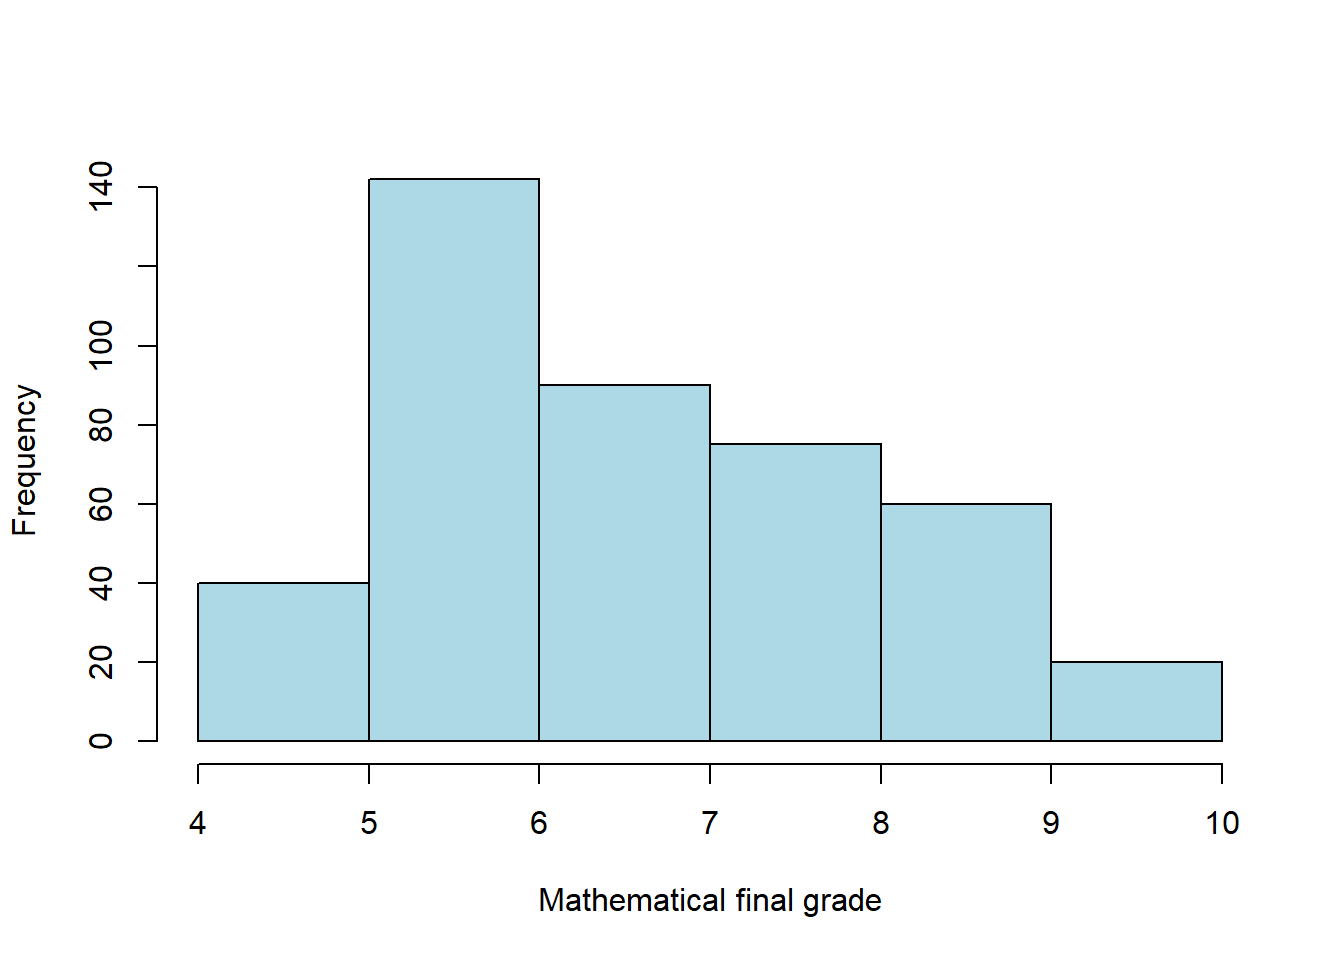
\includegraphics[width=0.30\textwidth]{math_final.png}
    \caption{Students' final mathematical grade distribution.}
    \label{fig:math}
\end{figure}

\begin{figure}[H]
    \centering
    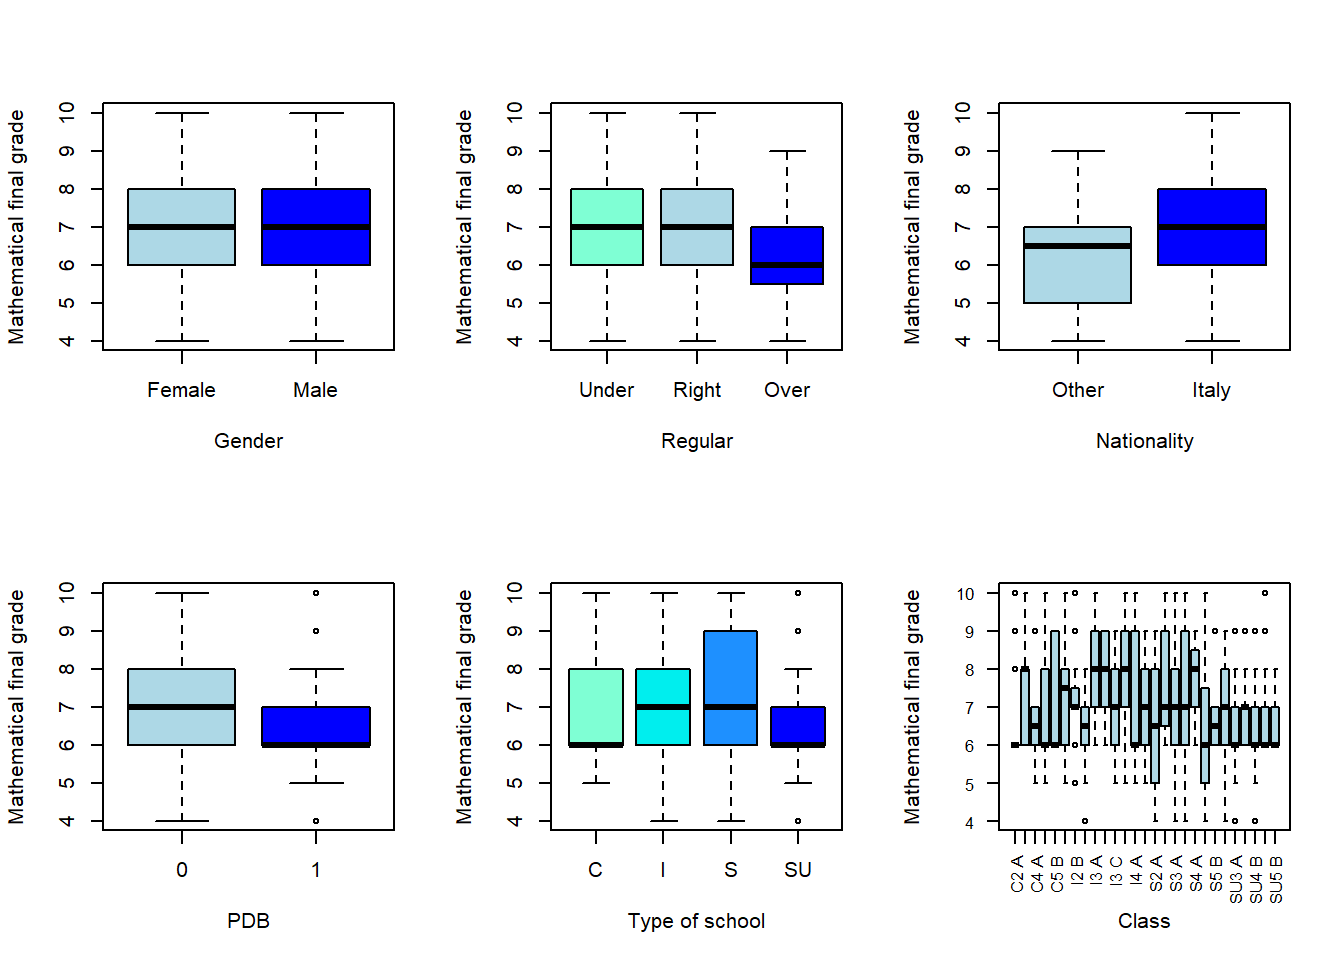
\includegraphics[width=0.75\textwidth]{boxplot_2.png}
    \caption{Comparison between \(gender, \, regular, \, nationality, \, PDB, \, type\,of\,school, \, class\) covariates and mathematical final evaluation.}
    \label{fig:box}
\end{figure}

\begin{figure}[H]
    \centering
    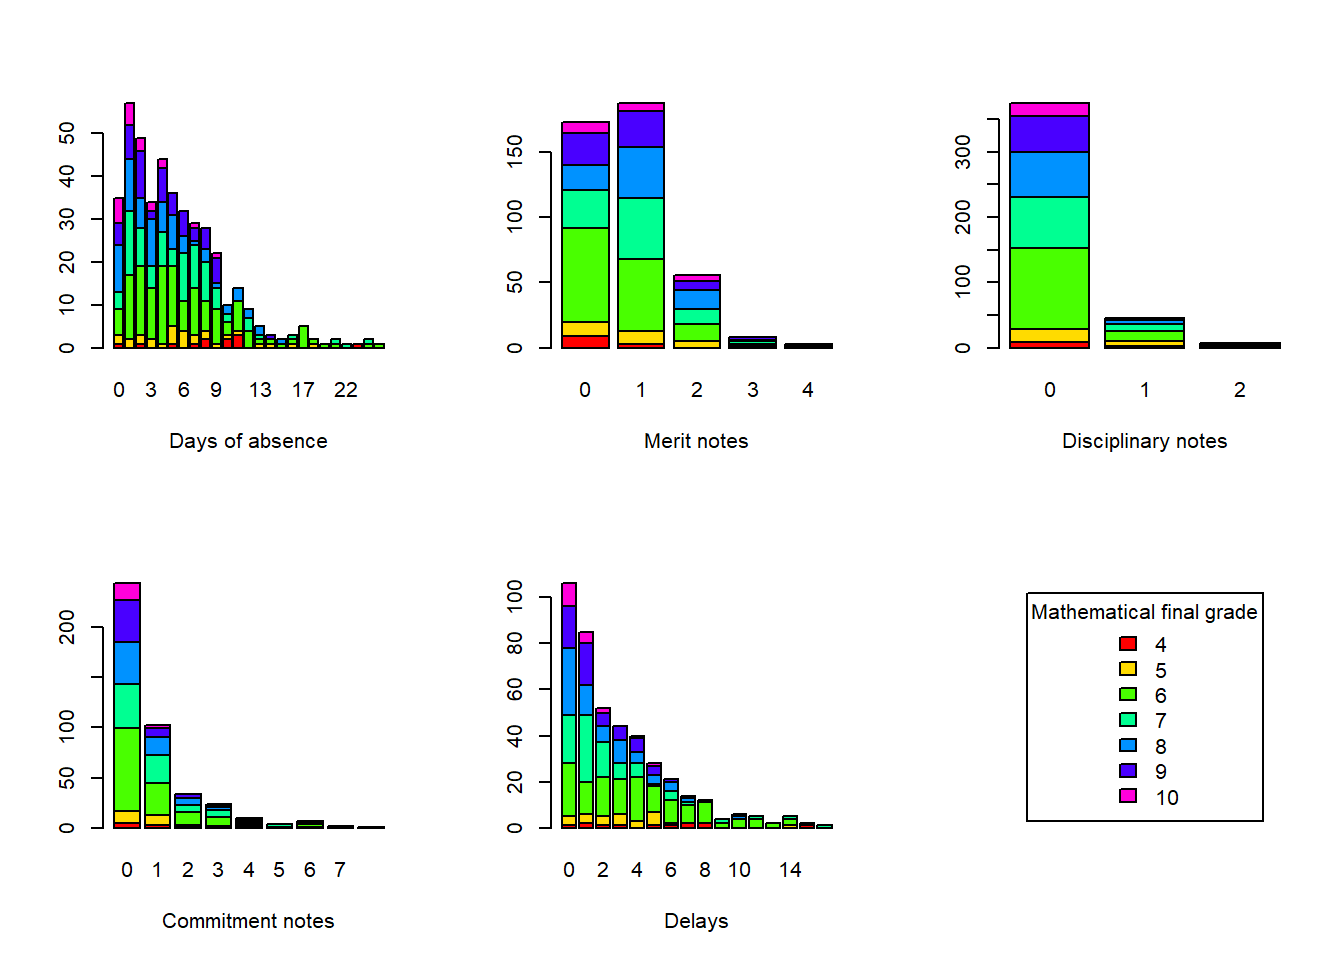
\includegraphics[width=0.8\textwidth]{assenze.png}
    \caption{Comparison between \(absence, \, merit\,notes, \, disciplinary\,notes, \, commitment\,notes, \, delays\) covariates and mathematical final evaluation.}
    \label{fig:ass}
\end{figure}







\subsection{Model results}
\label{sec:modres}
In the same way as in the simulation study, in order to evaluate the predictive performances of the four compared models, the dataset is randomly split into training and test sets, with a ratio of 80\% for training and 20\% for testing.

As mentioned in Section \ref{sec:dataset} two types of mixed-effects models are implemented: the first ones with ordinal response variable the student's final grade in mathematics, the others with ordinal response the created variable \(risk\).
For each collection of models three different set of covariates are tested:
\begin{itemize}
    \item all varaibles listed in Table \ref{table:fix_var}, excluding the ones related to the school performance in mathematics (i.e. \(first \, term \, math\), \(variance\), \(previous \, math \, grade\));
    \item all varaibles listed in Table \ref{table:fix_var}, excluding the ones related to the previous year school performance in mathematics (i.e. \(previous \, math \, grade\));
    \item all varaibles listed in Table \ref{table:fix_var}.
\end{itemize}
The choice of monitoring the differences among the three sets of covariates is done in order to observe the OMERF method's efficiency in various settings.
Indeed, the student's achievements in mathematics during the first half of the year and related to the previous year are expected to be highly linearly correlated with the model response.
The importance of this dependence with the target variable will greately influence the model estimates, and thus impact the model performances, probably favoring the simplest models, as emerged from the simulation study in Section \ref{sec:simres}.
For this reason, various combinations of variables are implemented with the aim of recording results even in a less strictly linear context and observing the behaviour of covariates that potentially have nonlinear trends.

In all these models a random intercept \(b_0\) for the student's class is included.

The prediction performances are reported in Tables \ref{table:res_math} and \ref{table:res_risk}.
From the results in Table \ref{table:res_math} it is clear that all the models exhibit poor predictive capabilities; this is probably due to the large number of levels of the considered response, which makes it difficult for models to distinguish between them.
In Table \ref{table:res_risk} in fact, having a three-level target variable, the performances are significantly better.
Moreover, it can be noticed that in the latter setting, in the first two cases implemented, the differences between all the models are subtler.
On the contrary, with the last set of covariates the rest of the models tend to overperform OMERF, sufficiently covering the level of complexity required by the problem. This phenomenon perfectly follows our previously stated hypothesis;
i.e. the information regarding the students' mathematical achievements has a linear relationship with the target values, and thus the existing models are best suited to this type of problem, reaching highest forecasting abilities when also the information concerning the 2017/2018 academic year is included.

Nevertheless, from OMERF's outputs can be retrieved meaningful information. Focusing on the second collection of models with \(risk\) response variable, all the three models highlight a similar hierarchical structure, as it is evident from the estimates of random intercepts shown in Figure \ref{fig:reff}.
Since the first model has less predictive power with respect to the other two, this reflectes in its lower ability to outline the nested structure; but it is in any case clear, even though less significant, the trend of random effects between classes.
Therefore, there is a visible difference in the performances of students belonging to different classes, as already noted in the exploratory analysis in Figure \ref{fig:box}. However, only a few classes have an intercepts significantly different from 0 (with 95\% confidence), deviating from the average.
In particular, there is not a recognisable pattern related to the age of the students in the classes or related to the different types of school. Instead, the class effect, net to the fixed effects contribution, might be due to having different teaching staff.

As the variance of the standard logistic distribution is \(\pi^2 / 3 \cong 3.29\), and the variance of the random effects in the three models are \(\sigma^2_{m4} = 0.5619,\quad \sigma^2_{m5} = 2.3345,\quad \sigma^2_{m6} = 1.8302\), the Intraclass Correlation Coefficients (ICCs) for the underlying linear
models can be estimated as:
\begin{gather*}
    \begin{aligned}
        ICC_4 = \frac{\sigma^2_{m4}}{\sigma^2_{m4}+\pi^2 / 3}= 0.1459, \quad ICC_5 = \frac{\sigma^2_{m5}}{\sigma^2_{m5}+\pi^2 / 3}= 0.4151, \quad ICC_6 = \frac{\sigma^2_{m6}}{\sigma^2_{m6}+\pi^2 / 3}= 0.3574.
    \end{aligned}
\end{gather*}
These values of ICC, measuring the unexplained variance in the response that can be atributed to the nested structure of students, together with the fact that some random intercepts are significantly different from zero (Figure \ref{fig:reff})
imply the existence of a substantial heterogeneity in the achievements among various classes. This highlight once again the importance of considering the hierarchical structure of these data.

\begin{figure}[H]
    \centering
    \subfloat[Model with all variables listed in Table \ref{table:fix_var}, excluding \(first \, term \, math\), \(variance\), \(previous \, math \, grade\).]{
        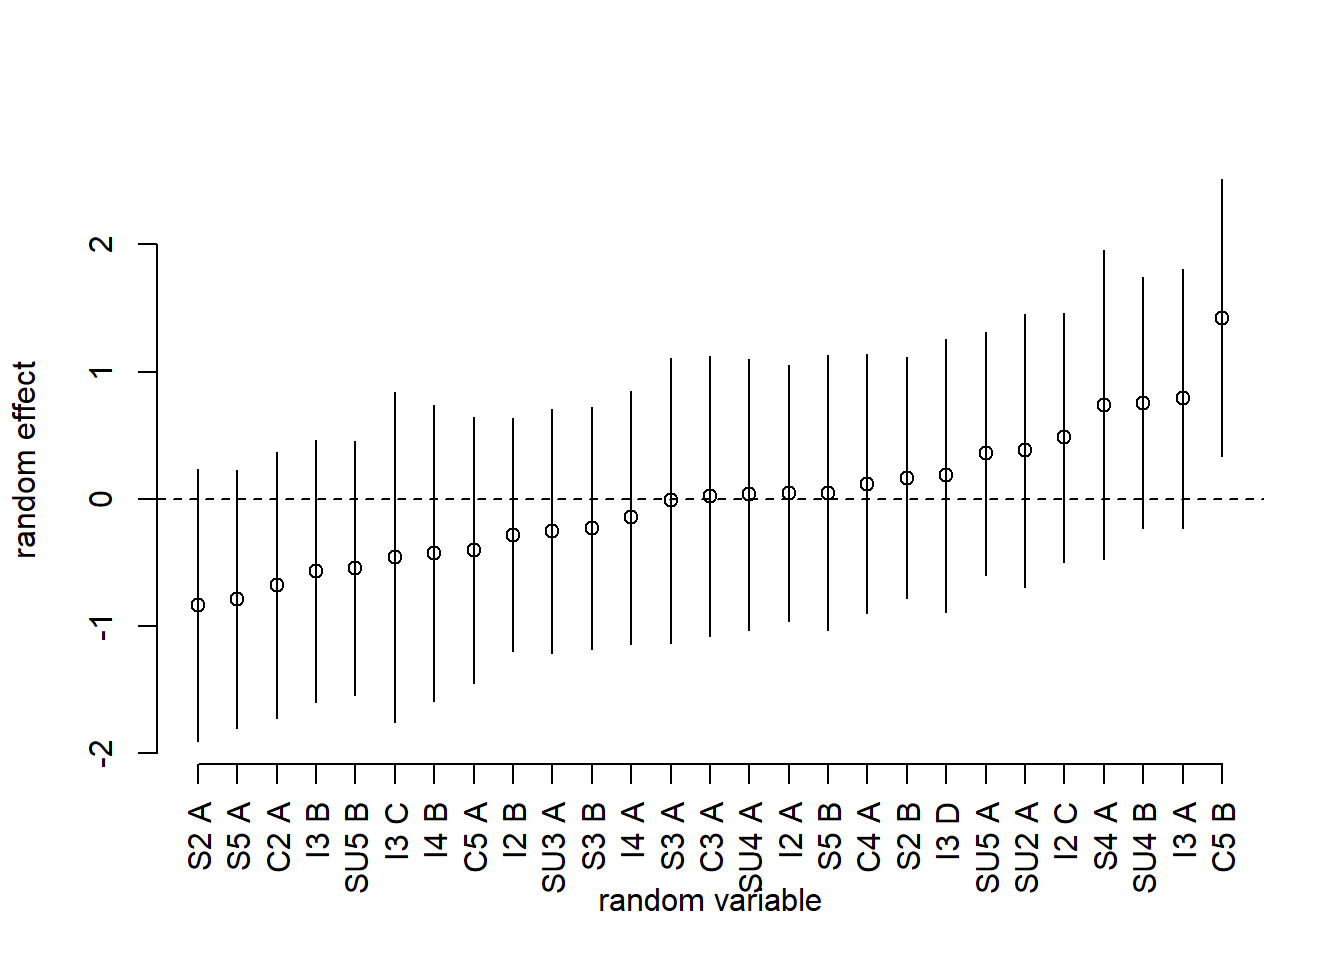
\includegraphics[scale=0.4]{Images/re0_3.png}
    }
    \quad
    \subfloat[Model with all variables listed in Table \ref{table:fix_var}, excluding \(previous \, math \, grade\).]{
        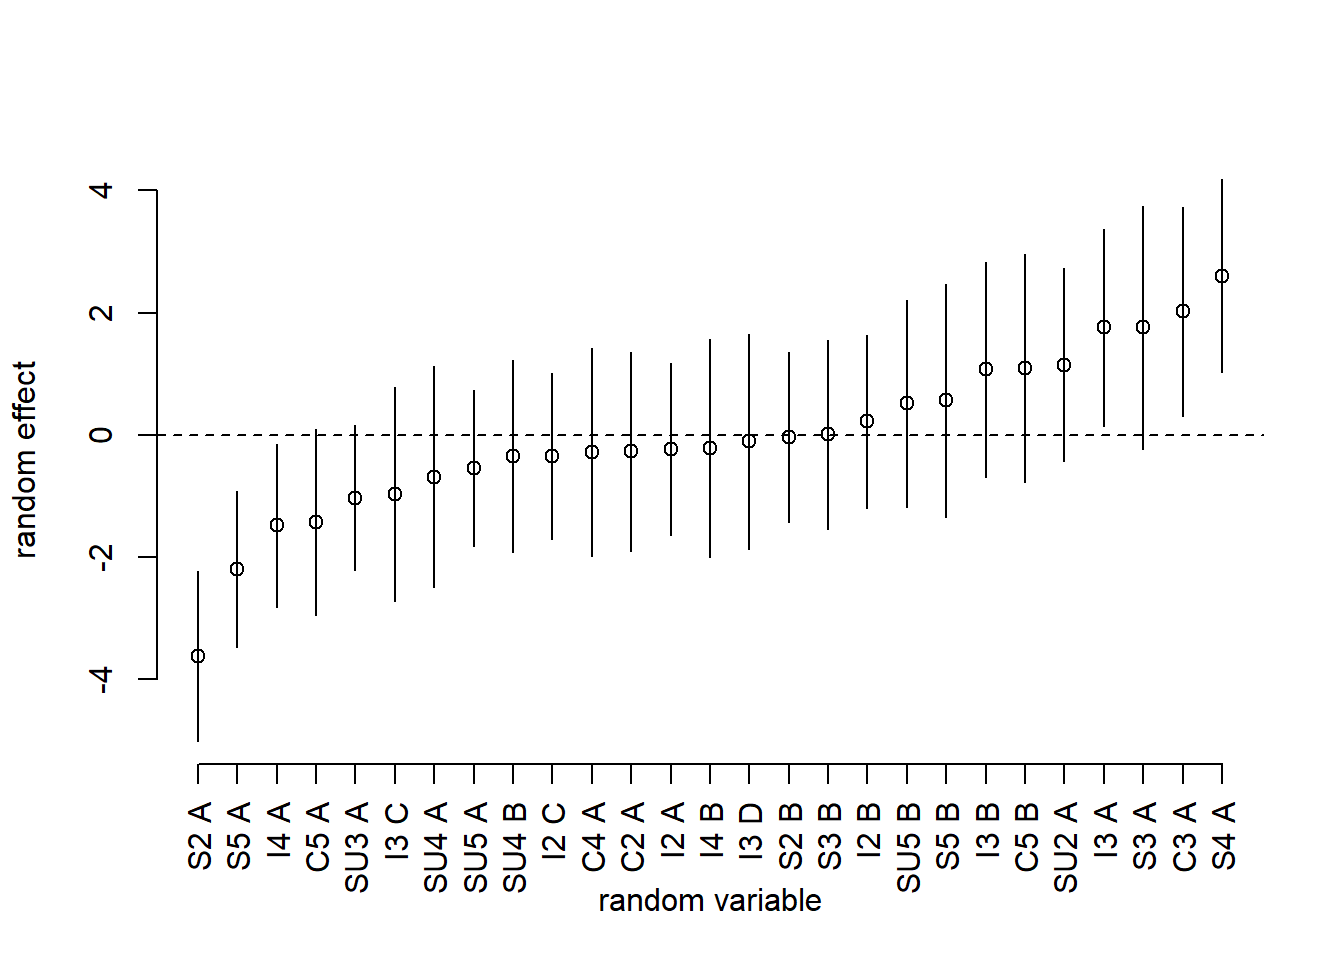
\includegraphics[scale=0.4]{Images/re1_3.png}
    }
    \quad
    \subfloat[Model with all variables listed in Table \ref{table:fix_var}.]{
        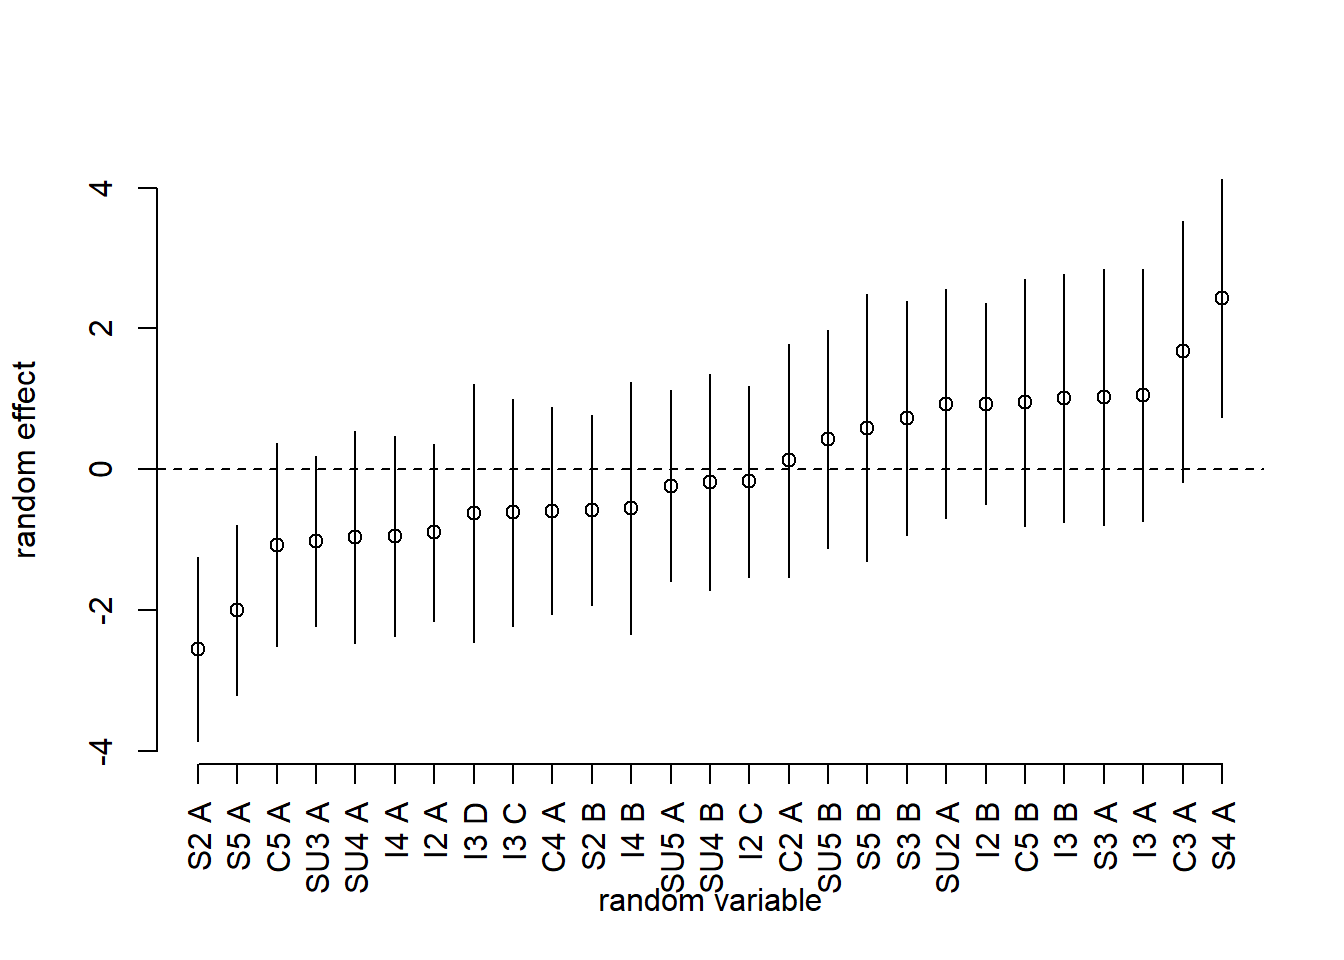
\includegraphics[scale=0.4]{Images/re2_3.png}
    }
    \caption[]{Random intercepts with their confidence intervals, relative to the 27 classes estimated by the OMERF model.}
    \label{fig:reff}
\end{figure}

Regarding the fixed effects, RF model in the OMERF algorithm measures the imporance of each covariate in explaining the response and the partial effect of each covariate.
Figure \ref{fig:varimp} shows dotcharts of the importance of the variables in the three models, as measured by two different indices.
The first index is derived from permuting out-of-bag data: for each tree, the prediction error (MSE for regression) on the out-of-bag portion of the data is recorded. Subsequently, the same process is repeated after permuting each predictor variable. The discrepancy between these two measures is then averaged across all trees comprising the random forest and normalized by the standard deviation of the differences.
The second index is the total decrease in node impurities resulting from splitting on the variable, averaged over all trees. In the context of regression, node impurity is quantified by the residual sum of squares.

As expected, when the covariates regarding mathematical performances are included in the models, they are of total importance, reducing the influence of others. In any case, the importance of the other covariates appears to be in line with what was evidenced by the boxplots in Figure \ref{fig:box}.
Specifically, by adding in the last two models the variables related to students' performance at school, the other covariates remain consistent, with \(absence\), \(delays\), \(PDB\) and \(tenuered \, teachers\) being generally the most important ones. This reflects the fact that even the first is a valid model despite having less predictive capabilities.

\begin{figure}[H]
    \centering
    \subfloat[Variable importance plot of the model with all variables listed in Table \ref{table:fix_var}, excluding \(first \, term \, math\), \(variance\), \(previous \, math \, grade\).]{
        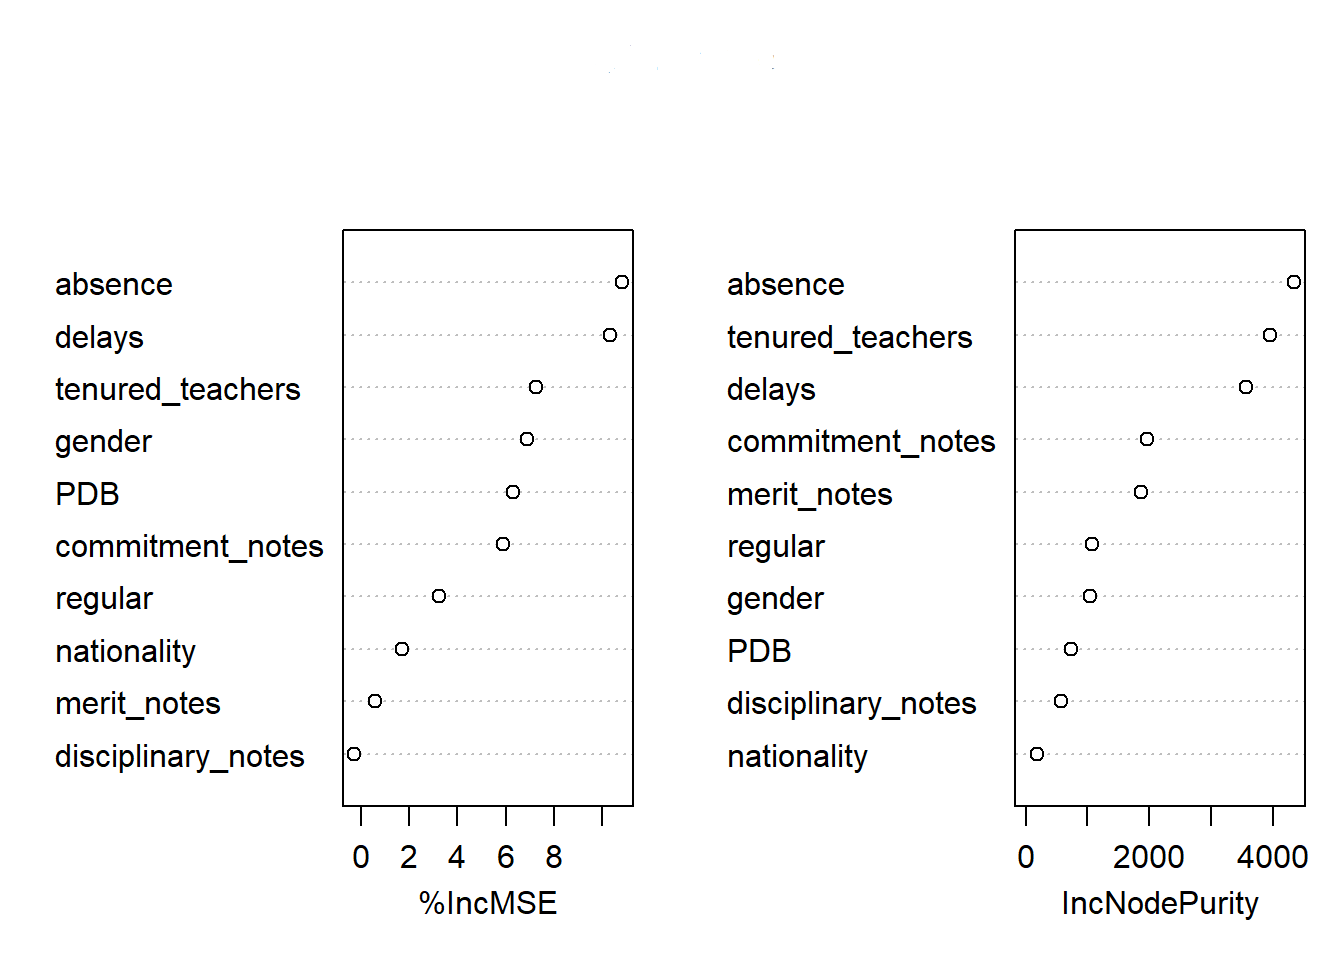
\includegraphics[scale=0.4]{Images/varimp0_2.png}
    }
    \quad
    \subfloat[Variable importance plot of the model with all variables listed in Table \ref{table:fix_var}, excluding \(previous \, math \, grade\).]{
        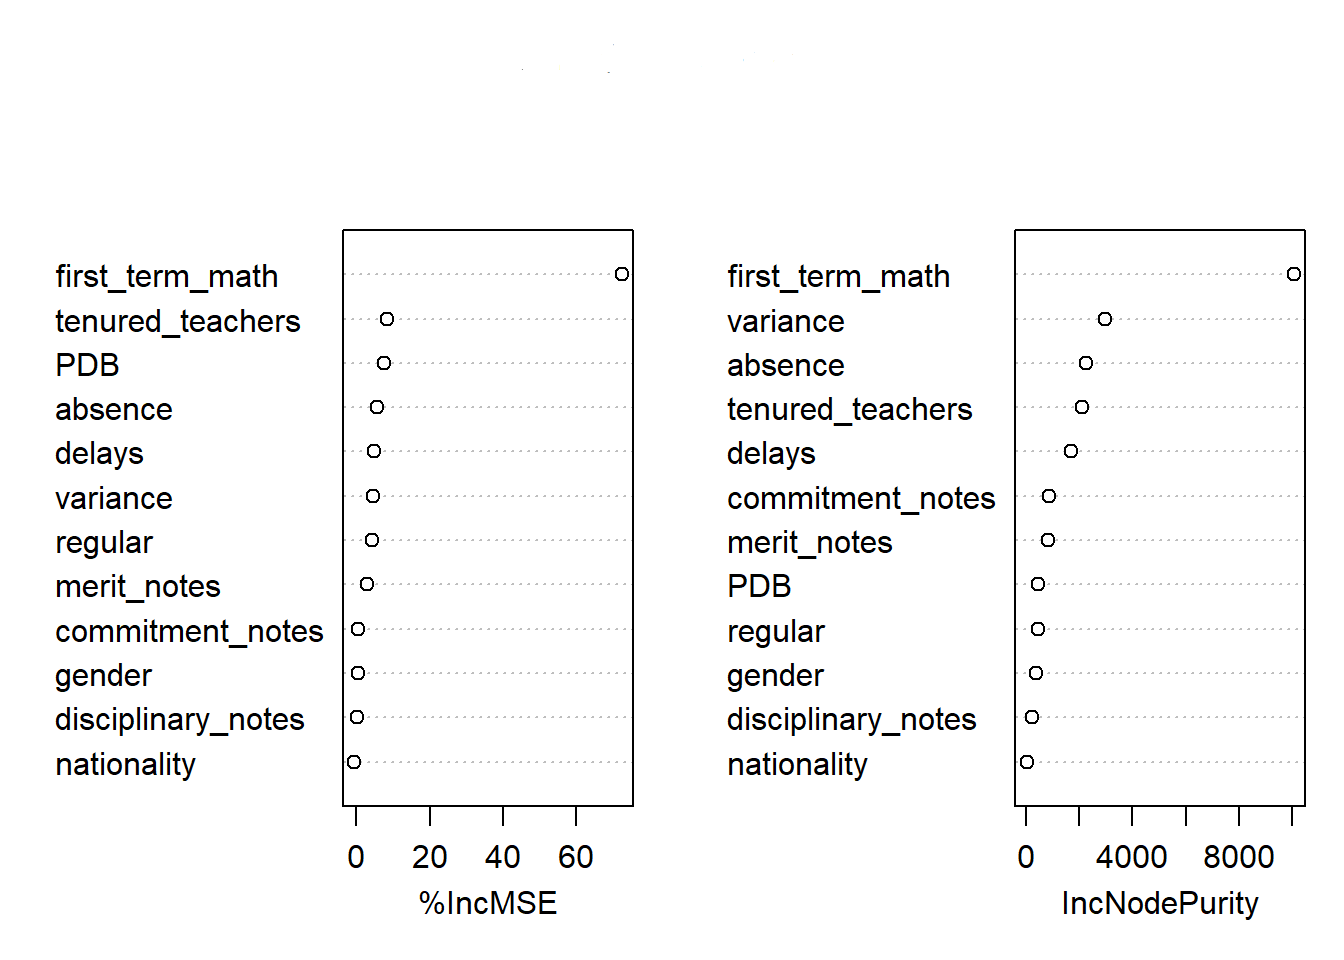
\includegraphics[scale=0.4]{Images/varimp1_2.png}
    }
    \quad
    \subfloat[Variable importance plot of the model with all variables listed in Table \ref{table:fix_var}.]{
        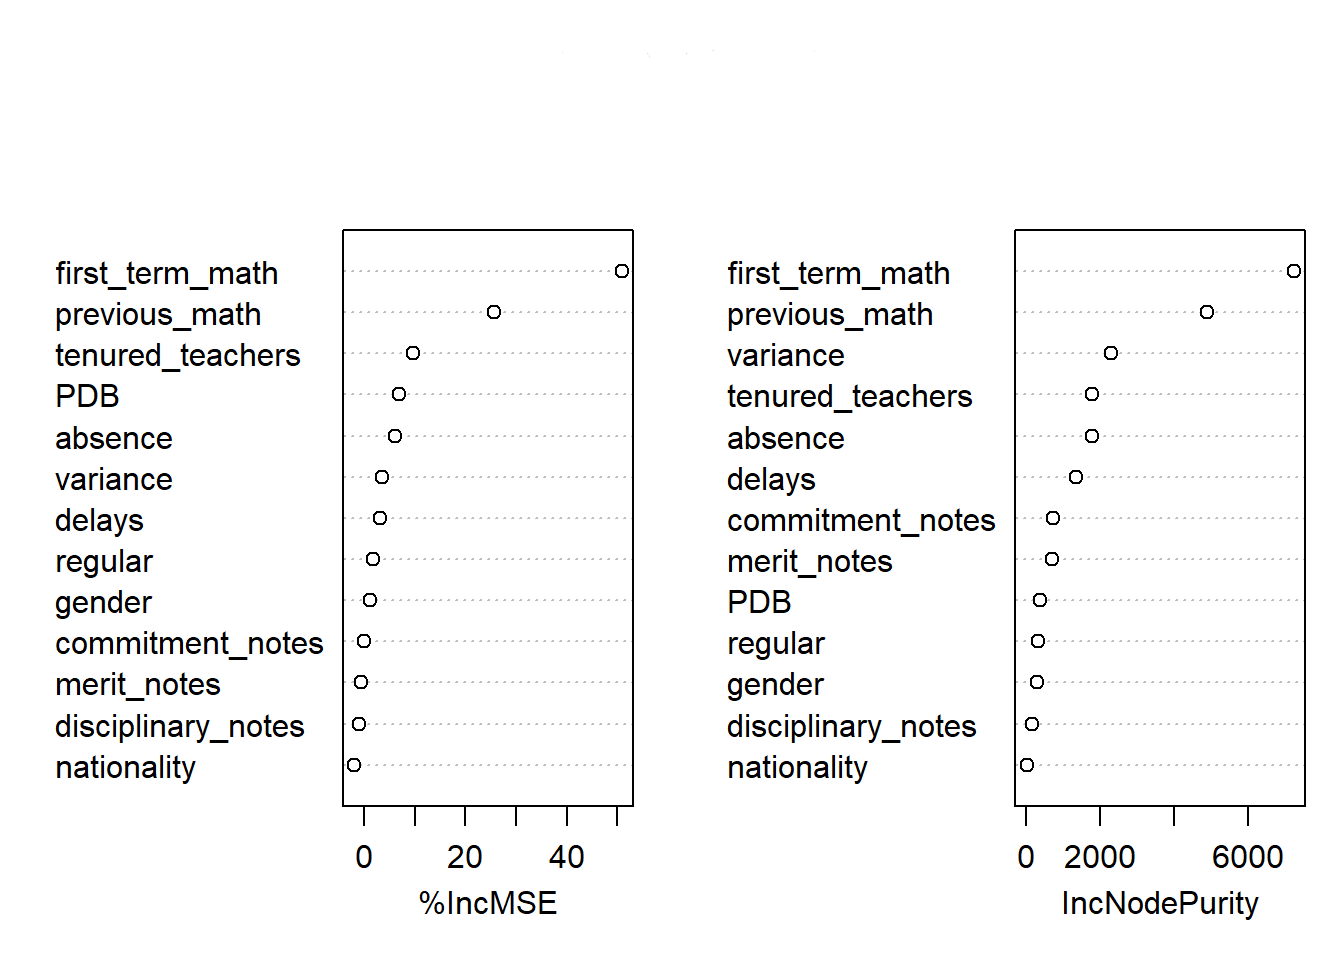
\includegraphics[scale=0.4]{Images/varimp2_2.png}
    }
    \caption[]{Dotcharts of the importance of the fixed variables used in OMERF models in explaining the response.}
    \label{fig:varimp}
\end{figure}

The importance plot for variables identifies significant covariates but does not provide insights into the nature of their relationship with the response variable.
Partial plots, on the other hand, offer a clearer view of how each covariate is associated with the target variable, net to the other covariates included in the model.
Figures \ref{fig:fe0}, \ref{fig:fe1} and \ref{fig:fe2} display partial plots for all continuous and categorical fixed-effect covariates, in each implemented model.

These plots highlight some common patterns: \(absence\) and \(delays\) show an inverse proportional association with the response; on the contrary \(merit \, notes\), \(commitment \, notes\) and obviously \(first \, term \, math\) and \(previous \, math \, grade\) are directly proportional to it;
finally the factor covariates seem to have little to no influence on the target, especially in the last two models.

\begin{figure}[H]
    \centering
    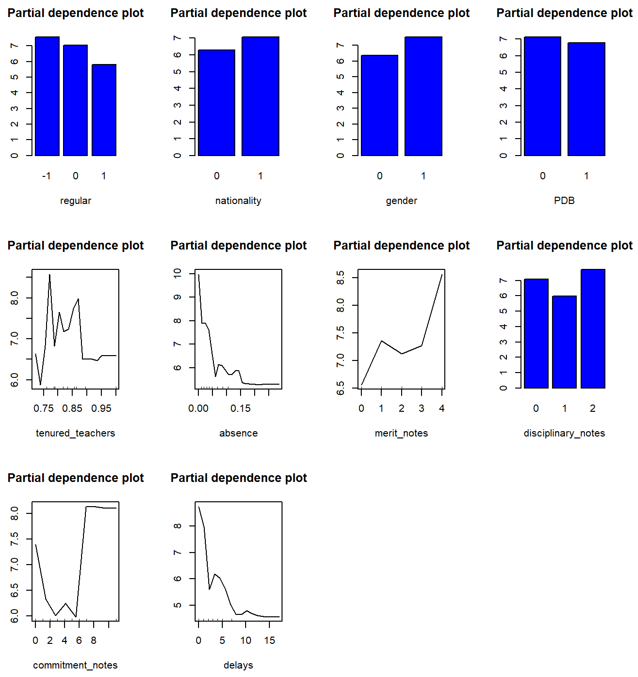
\includegraphics[width=0.61\textwidth]{fe0_2.png}
    \caption{Partial plots of the RF target variable in OMERF method with respect to the covariates of the model with all varaibles listed in Table \ref{table:fix_var}, excluding \(first \, term \, math\), \(variance\), \(previous \, math \, grade\).}
    \label{fig:fe0}
\end{figure}

\begin{figure}[H]
    \centering
    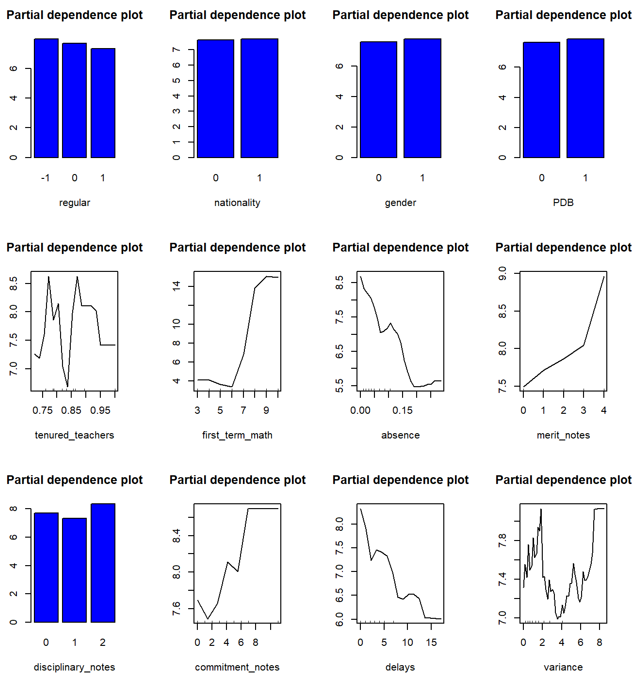
\includegraphics[width=0.61\textwidth]{fe1_2.png}
    \caption{Partial plots of the RF target variable in OMERF method with respect to the covariates of the model with all varaibles listed in Table \ref{table:fix_var}, excluding \(previous \, math \, grade\).}
    \label{fig:fe1}
\end{figure}

\begin{figure}[H]
    \centering
    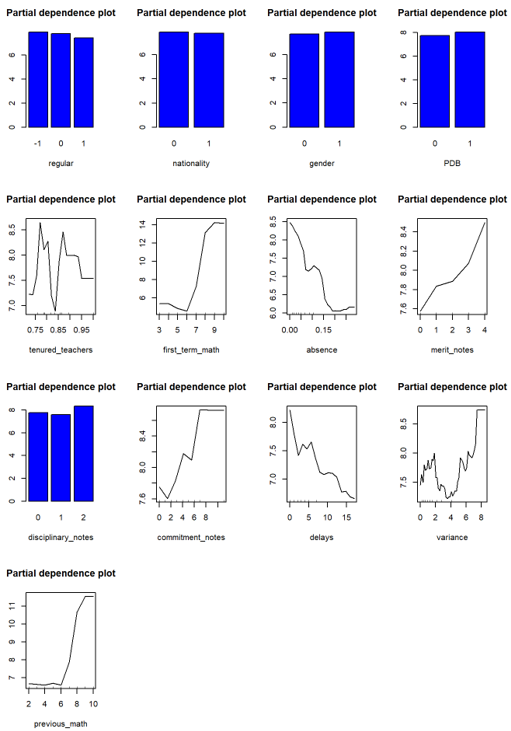
\includegraphics[width=0.61\textwidth]{fe2_2.png}
    \caption{Partial plots of the RF target variable in OMERF method with respect to the covariates of the model with all varaibles listed in Table \ref{table:fix_var}.}
    \label{fig:fe2}
\end{figure}

A potential limitation of the OMERF algorithm stems from the initial step where, during the first initialization, the method estimates the target values (\(\eta_{ijc}\)) through a CLM.
This model imposes a linear effect of covariates on a transformation of the response thereby potentially losing the intricacies that the random forest could capture in the subsequent step of the algorithm.

For this reason a second version of OMERF is implemented, in which the interactions between all covariates and their squares are added to the CLM formula. The resulting performance measures are summarized in Table \ref{table:omerf2}.
The results are better with respect to the previous version and this could be a hint for further developments.

In conclusion, this dataset does not fully justify the use of a method like OMERF, which works more effectively and advantageously in problems with a higher level of complexity.
However, we have received confirmation of how we expected the algorithm to behave, and it is evident that OMERF method is still able to extract additional meaningful insights from the phenomenon under analysis and information on potential nonlinearities.

\begin{table}[H]
    \centering 
    \begin{tabular}{|p{1em} c c c c c c c |}
    \hline
    \rowcolor{bluePoli!40}
    & \textbf{Model} & \textbf{Acc} & \textbf{MSE} & \textbf{ARI} & \textbf{Cohen's k} & \textbf{Cardoso} & \textbf{Ballante} \T\B \\
    \hline \hline
    \textbf{1} & clm & 0.3452 & 2.8571 & 0.0319 & 0.0802 & 0.7309 & 0.2085 \T\B \\
    \textbf{1} & clmm & 0.3690  & $\textcolor{bluePoli}{2.8214}$ & 0.0501 & 0.1121 & 0.7212 & 0.2146 \T\B \\
    \textbf{1} & ordforest & $\textcolor{bluePoli}{0.4405}$ & 43.2738 & $\textcolor{bluePoli}{0.0788}$ & $\textcolor{bluePoli}{0.2229}$ & $\textcolor{bluePoli}{0.6738}$ & $\textcolor{bluePoli}{0.1666}$ \T\B \\
    \textbf{1} & omerf & 0.2976 & 3.3333 & -0.0210 & 0.0012 & 0.7644 & 0.2404 \T\B \\
    \hline
    \textbf{2} & clm & 0.4286 & 1.0238 & 0.1640 & 0.2526 & 0.6096 & 0.1685 \T\B \\
    \textbf{2} & clmm & 0.4286  & $\textcolor{bluePoli}{0.9048}$ & 0.1569 & 0.2532 & $\textcolor{bluePoli}{0.6005}$ & 0.1625 \T\B \\
    \textbf{2} & ordforest & $\textcolor{bluePoli}{0.4762}$ & 36.3929 & $\textcolor{bluePoli}{0.2226}$ & $\textcolor{bluePoli}{0.3046}$ & 0.6021 & $\textcolor{bluePoli}{0.1327}$ \T\B \\
    \textbf{2} & omerf & 0.3571 & 1.9643 & 0.0806 & 0.0836 & 0.6558 & 0.1761 \T\B \\
    \hline
    \textbf{3} & clm & 0.4643 & 0.9167 & 0.1701 & 0.3019 & 0.5839 & 0.1546 \T\B \\
    \textbf{3} & clmm & $\textcolor{bluePoli}{0.5357}$  & $\textcolor{bluePoli}{0.8095}$ & 0.2227 & $\textcolor{bluePoli}{0.3974}$ & $\textcolor{bluePoli}{0.5327}$ & 0.1244 \T\B \\
    \textbf{3} & ordforest & 0.5238 & 36.6429  & $\textcolor{bluePoli}{0.2510}$ & 0.3682 & 0.5563  & $\textcolor{bluePoli}{0.1199}$ \T\B \\
    \textbf{3} & omerf & 0.4048 & 1.7024 & 0.0846 & 0.1559 & 0.6239 & 0.1615 \B \\
    \hline
    \end{tabular}
    \\[10pt]
    \caption{Prediction performances of the four methods in each model listed in Table \ref{table:fix_var}, with ordinal reponse variable the final mathematical grade.}
    \label{table:res_math}
\end{table}


\begin{table}[H]
    \centering 
    \begin{tabular}{|p{1em} c c c c c c c |}
    \hline
    \rowcolor{bluePoli!40}
    & \textbf{Model} & \textbf{Acc} & \textbf{MSE} & \textbf{ARI} & \textbf{Cohen's k} & \textbf{Cardoso} & \textbf{Ballante} \T\B \\
    \hline \hline
    \textbf{4} & clm & 0.4706 & 0.6000 & -0.0065 & -0.0037 & 0.6147 & 0.3859 \T\B \\
    \textbf{4} & clmm & 0.5059 & 0.5294 & -0.0039 & 0.0346 & 0.5688 & 0.3723 \T\B \\
    \textbf{4} & ordforest & $\textcolor{bluePoli}{0.5529}$ & $\textcolor{bluePoli}{0.4471}$ & 0.00002 & 0.1247 & $\textcolor{bluePoli}{0.5212}$ & $\textcolor{bluePoli}{0.2561}$ \T\B \\
    \textbf{4} & omerf & 0.5412 & 0.5294 & $\textcolor{bluePoli}{0.0213}$  & $\textcolor{bluePoli}{0.1487}$ & 0.5609 & 0.3411 \T\B\\
    \hline
    \textbf{5} & clm & 0.6471 & 0.3529 & 0.1326 & 0.3390 & 0.4318 & 0.2309 \T\B \\
    \textbf{5} & clmm & $\textcolor{bluePoli}{0.6588}$ & $\textcolor{bluePoli}{0.3412}$ & $\textcolor{bluePoli}{0.1575}$ & $\textcolor{bluePoli}{0.3647}$ & 0.4259 & 0.2181 \T\B \\
    \textbf{5} & ordforest & $\textcolor{bluePoli}{0.6588}$ & $\textcolor{bluePoli}{0.3412}$ & 0.1263 & 0.3293 & $\textcolor{bluePoli}{0.4128}$ & $\textcolor{bluePoli}{0.1743}$ \T\B \\
    \textbf{5} & omerf & 0.6471 & 0.3529 & 0.1176 & 0.3241 & 0.4361 & 0.2256 \T\B\\
    \hline
    \textbf{6} & clm & 0.7294 & $\textcolor{bluePoli}{0.2706}$ & 0.2925 & 0.4991 & 0.3484 & 0.1808 \T\B \\
    \textbf{6} & clmm & 0.7176 & 0.2824 & 0.2650 & 0.4863 & 0.3689 & $\textcolor{bluePoli}{0.1684}$ \T\B \\
    \textbf{6} & ordforest & 0.7294 & $\textcolor{bluePoli}{0.2706}$ & 0.2686 & 0.4713 & 0.3338 & 0.1812 \T\B \\
    \textbf{6} & omerf & $\textcolor{bluePoli}{0.7529}$ & 0.2824 & $\textcolor{bluePoli}{0.3339}$ & $\textcolor{bluePoli}{0.5193}$ & $\textcolor{bluePoli}{0.3179}$ & 0.1818 \B\\
    \hline
    \end{tabular}
    \\[10pt]
    \caption{Prediction performances of the four methods in each model listed in Table \ref{table:fix_var}, with ordinal reponse variable the created variable \(risk\).}
    \label{table:res_risk}
\end{table}

\begin{table}[H]
    \centering 
    \begin{tabular}{|p{1em} c c c c c c c |}
    \hline
    \rowcolor{bluePoli!40}
    & \textbf{Model} & \textbf{Acc} & \textbf{MSE} & \textbf{ARI} & \textbf{Cohen's k} & \textbf{Cardoso} & \textbf{Ballante} \T\B \\
    \hline \hline
    \textbf{4} & omerf new & 0.5529 & 0.6588 &  0.0719 & 0.2444 & 0.5755 & 0.3320 \T\B \\
    \hline
    \textbf{5} & omerf new & 0.6824 & 0.3176 & 0.1998 & 0.4219 & 0.4144 & 0.2013 \T\B \\
    \hline
    \textbf{6} & omerf new & 0.7176 & 0.2824 & 0.2536 & 0.4842 & 0.3737 & 0.1722 \B \\
    \hline
    \end{tabular}
    \\[10pt]
    \caption{Prediction performances of the new version of OMERF method in each model listed in Table \ref{table:fix_var}, with ordinal reponse variable the created variable \(risk\).}
    \label{table:omerf2}
\end{table}



